\section{ChimeraX Restore Session protocol}
\label{app:chimeraRestoreSession}%a030

Protocol designed to restore \chimera session, provided that this session has been saved previously in \scipion. Currently, four protocols save \chimera sessions when \chimera commands \ttt{scipionwrite}, \ttt{scipionss} or \ttt{scipioncombine} are used, \scommand{chimerax - rigid fit}, \scommand{chimerax - operate}, \scommand{chimerax - model from template} and \scommand{chimerax - map subtraction} (Appendices \ref{app:chimeraRigidFit}, \ref{app:chimeraOperate}, \ref{app:modelFromTemplate} and \ref{app:chimeraMapSubtraction}, respectively). Restored sessions allow inspect any element contained in a previously saved \chimera session, perform \chimera operations, and finally save maps or atomic structures.

 \begin{itemize}
  \item Requirements to run this protocol and visualize results:
    \begin{itemize}
        \item \scipion plugin: \ttt{scipion-em}
        \item \scipion plugin: \ttt{scipion-em-chimera}
    \end{itemize}
  \item \scipion menu:\\
   \ttt{Model building -> Tools-Calculators} (\ffigure{fig:app_protocol_chimera_3} (A))
  
  \item Protocol form parameters (\ffigure{fig:app_protocol_chimera_3} (B)):
  
    \begin{figure}[H]
     \centering 
     \captionsetup{width=.7\linewidth} 
     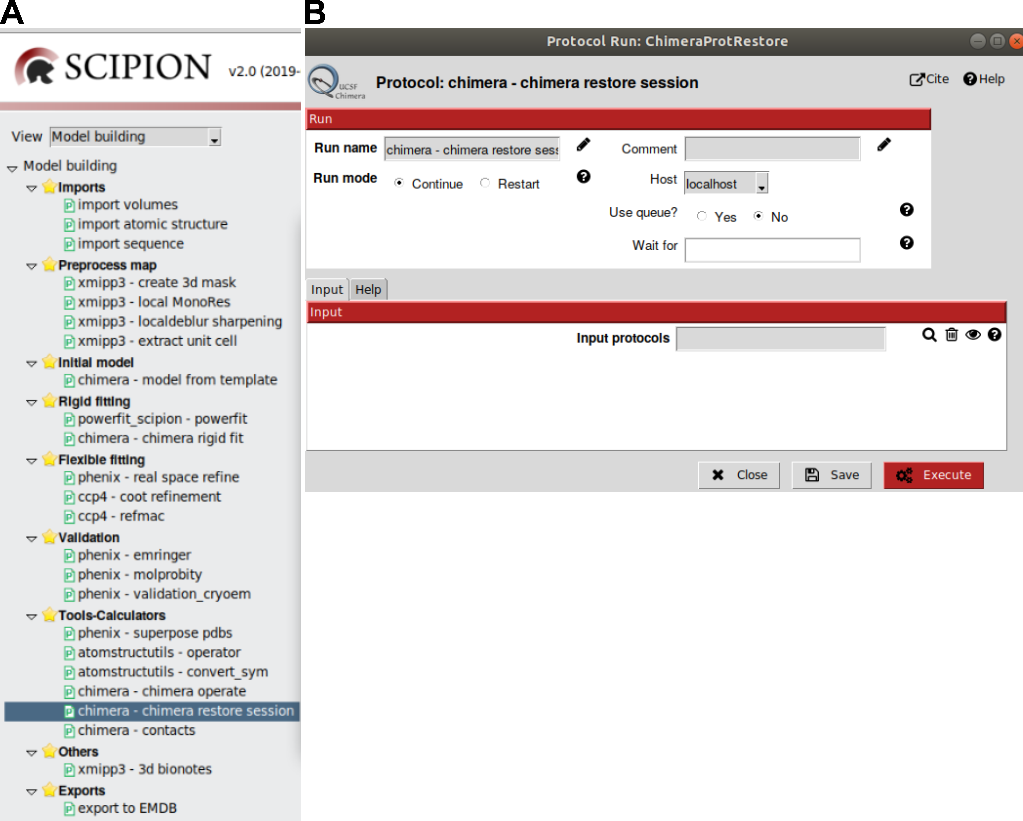
\includegraphics[width=0.90\textwidth]{Images_appendix/Fig118.pdf}
     \caption{Protocol \scommand{chimerax - restore session}. A: Protocol location in \scipion menu. B: Protocol form.}
     \label{fig:app_protocol_chimera_3}
    \end{figure}
    
    \begin{itemize}
     \item \ttt{Input} section

    \begin{itemize}
     \item \ttt{Input protocols}: Parameter that allows to select a particular protocol in which \chimera session has been saved in \scipion. As it was mentioned before, four protocols support this possibility (\chimera \ttt{rigid fit}, \chimera \ttt{operate}, \chimera \ttt{model from template} and \chimera \ttt{map subtraction}).
     
    \end{itemize}
    \item \ttt{Help} section
    
    This section contains \chimera commands required to save $models$ according to their reference volumes, which can also be saved if required. Remark that using \ttt{scipionwrite} or \ttt{scipioncombine} commands, \chimera session will be saved by default, without prejudice that it may be saved with \ttt{scipionss} command. \chimera sessions can be restored again by using this same \scommand{chimerax - restore session} protocol.
    
    \end{itemize}

  \item Protocol execution:
  
  Adding specific protocol label is recommended in \ttt{Run name} section, at the form top. To add the label, open the protocol form, press the pencil symbol at the right side of \ttt{Run name} box, complete the label in the new opened window, press OK and, finally, close the protocol. This label will be shown in the output summary content (see below). If you want to run again this protocol, do not forget to set to \ttt{Restart} the \ttt{Run mode}.\\
  Press the \ttt{Execute} red button at the form bottom.\\
  
  \chimera graphics window will be opened after executing the protocol showing the complete list of elements that appeared in \chimera graphics window when the session was saved, coordinate axes, electron density maps, and atomic structures. Steps to follow depend on the specific operation to carry out. New volumes or structures may be generated as usual in \chimera, and they can be saved in \scipion in the common way.
  \begin{itemize}
   
   \item To save a map or an atomic structure generated with this protocol:
   Write in \chimera command line:\\
   \ttt{scipionwrite \#n prefix userString\_}.\\Replace \ttt{\#n} by model numbers shown in \chimera \ttt{Models} panel. \ttt{prefix} + string preferred by the user to easily identify the atomic structure is optional, although quite recomendable.\\
   Replace \ttt{\#n} by model numbers shown in \chimera \ttt{Models} panel. 
   
   \item Close \chimera graphics window.

 \end{itemize}
  \item Visualization of protocol results:
  
    After executing the protocol, press \ttt{Analyze Results} and \chimera graphics window will be opened by default. Atomic structures and volumes are referred to the origin of coordinates in \chimera. To show the relative position of atomic structure and electron density volume, the three coordinate axes are represented; X axis (red), Y axis (yellow), and Z axis (blue) (\ffigure{fig:app_protocol_volume_3}). In this particular case a \chimera graphics window identical to the input session will be opened and it will include every element saved lately. 
   
  \item Summary content:
  
   \begin{itemize}
    \item If an atomic structure is generated:

    \begin{itemize}
     \item Protocol output (below \scipion framework):
      \ttt{chimerax - restore session -> Atom\_struct\_name};\\ \ttt{AtomStruct (pseudoatoms=True/ False, volume=True/ False)}.\\Pseudoatoms is set to \ttt{True} when the structure is made of pseudoatoms instead of atoms. Volume is set to \ttt{True} when an electron density map is associated to the atomic structure.\\
     \item \ttt{SUMMARY} box:\\Produced files:\\we have some result
    \end{itemize}
    \item If a volume is generated:
    
    \begin{itemize}
     \item Protocol output (below \scipion framework):
      \ttt{chimerax - restore session -> Map\_name};\\ \ttt{Volume (x, y, and z dimensions, sampling rate)}.\\
     \item \ttt{SUMMARY} box:\\Produced files:\\name of the map file\\we have some result
    \end{itemize}
    
   \end{itemize}
  
 \end{itemize}
